% Options for packages loaded elsewhere
% Options for packages loaded elsewhere
\PassOptionsToPackage{unicode}{hyperref}
\PassOptionsToPackage{hyphens}{url}
\PassOptionsToPackage{dvipsnames,svgnames,x11names}{xcolor}
%
\documentclass[
  spanish,
  14pt,
  letterpaper,
  DIV=11,
  numbers=noendperiod]{scrartcl}
\usepackage{xcolor}
\usepackage{amsmath,amssymb}
\setcounter{secnumdepth}{-\maxdimen} % remove section numbering
\usepackage{iftex}
\ifPDFTeX
  \usepackage[T1]{fontenc}
  \usepackage[utf8]{inputenc}
  \usepackage{textcomp} % provide euro and other symbols
\else % if luatex or xetex
  \usepackage{unicode-math} % this also loads fontspec
  \defaultfontfeatures{Scale=MatchLowercase}
  \defaultfontfeatures[\rmfamily]{Ligatures=TeX,Scale=1}
\fi
\usepackage{lmodern}
\ifPDFTeX\else
  % xetex/luatex font selection
\fi
% Use upquote if available, for straight quotes in verbatim environments
\IfFileExists{upquote.sty}{\usepackage{upquote}}{}
\IfFileExists{microtype.sty}{% use microtype if available
  \usepackage[]{microtype}
  \UseMicrotypeSet[protrusion]{basicmath} % disable protrusion for tt fonts
}{}
\makeatletter
\@ifundefined{KOMAClassName}{% if non-KOMA class
  \IfFileExists{parskip.sty}{%
    \usepackage{parskip}
  }{% else
    \setlength{\parindent}{0pt}
    \setlength{\parskip}{6pt plus 2pt minus 1pt}}
}{% if KOMA class
  \KOMAoptions{parskip=half}}
\makeatother
% Make \paragraph and \subparagraph free-standing
\makeatletter
\ifx\paragraph\undefined\else
  \let\oldparagraph\paragraph
  \renewcommand{\paragraph}{
    \@ifstar
      \xxxParagraphStar
      \xxxParagraphNoStar
  }
  \newcommand{\xxxParagraphStar}[1]{\oldparagraph*{#1}\mbox{}}
  \newcommand{\xxxParagraphNoStar}[1]{\oldparagraph{#1}\mbox{}}
\fi
\ifx\subparagraph\undefined\else
  \let\oldsubparagraph\subparagraph
  \renewcommand{\subparagraph}{
    \@ifstar
      \xxxSubParagraphStar
      \xxxSubParagraphNoStar
  }
  \newcommand{\xxxSubParagraphStar}[1]{\oldsubparagraph*{#1}\mbox{}}
  \newcommand{\xxxSubParagraphNoStar}[1]{\oldsubparagraph{#1}\mbox{}}
\fi
\makeatother

\usepackage{color}
\usepackage{fancyvrb}
\newcommand{\VerbBar}{|}
\newcommand{\VERB}{\Verb[commandchars=\\\{\}]}
\DefineVerbatimEnvironment{Highlighting}{Verbatim}{commandchars=\\\{\}}
% Add ',fontsize=\small' for more characters per line
\usepackage{framed}
\definecolor{shadecolor}{RGB}{46,52,64}
\newenvironment{Shaded}{\begin{snugshade}}{\end{snugshade}}
\newcommand{\AlertTok}[1]{\textcolor[rgb]{1.00,0.33,0.33}{\textbf{#1}}}
\newcommand{\AnnotationTok}[1]{\textcolor[rgb]{0.46,0.44,0.37}{#1}}
\newcommand{\AttributeTok}[1]{\textcolor[rgb]{0.98,0.15,0.45}{#1}}
\newcommand{\BaseNTok}[1]{\textcolor[rgb]{0.68,0.51,1.00}{#1}}
\newcommand{\BuiltInTok}[1]{\textcolor[rgb]{0.40,0.85,0.94}{#1}}
\newcommand{\CharTok}[1]{\textcolor[rgb]{0.90,0.86,0.45}{#1}}
\newcommand{\CommentTok}[1]{\textcolor[rgb]{0.46,0.44,0.37}{#1}}
\newcommand{\CommentVarTok}[1]{\textcolor[rgb]{0.46,0.44,0.37}{#1}}
\newcommand{\ConstantTok}[1]{\textcolor[rgb]{0.68,0.51,1.00}{#1}}
\newcommand{\ControlFlowTok}[1]{\textcolor[rgb]{0.98,0.15,0.45}{#1}}
\newcommand{\DataTypeTok}[1]{\textcolor[rgb]{0.40,0.85,0.94}{\textit{#1}}}
\newcommand{\DecValTok}[1]{\textcolor[rgb]{0.68,0.51,1.00}{#1}}
\newcommand{\DocumentationTok}[1]{\textcolor[rgb]{0.46,0.44,0.37}{#1}}
\newcommand{\ErrorTok}[1]{\textcolor[rgb]{1.00,0.33,0.33}{\underline{#1}}}
\newcommand{\ExtensionTok}[1]{\textcolor[rgb]{0.65,0.89,0.18}{\textbf{#1}}}
\newcommand{\FloatTok}[1]{\textcolor[rgb]{0.68,0.51,1.00}{#1}}
\newcommand{\FunctionTok}[1]{\textcolor[rgb]{0.65,0.89,0.18}{#1}}
\newcommand{\ImportTok}[1]{\textcolor[rgb]{0.98,0.15,0.45}{#1}}
\newcommand{\InformationTok}[1]{\textcolor[rgb]{0.95,0.98,0.55}{#1}}
\newcommand{\KeywordTok}[1]{\textcolor[rgb]{0.98,0.15,0.45}{#1}}
\newcommand{\NormalTok}[1]{\textcolor[rgb]{0.97,0.97,0.95}{#1}}
\newcommand{\OperatorTok}[1]{\textcolor[rgb]{0.97,0.97,0.95}{#1}}
\newcommand{\OtherTok}[1]{\textcolor[rgb]{0.65,0.89,0.18}{#1}}
\newcommand{\PreprocessorTok}[1]{\textcolor[rgb]{0.98,0.15,0.45}{#1}}
\newcommand{\RegionMarkerTok}[1]{\textcolor[rgb]{0.46,0.44,0.37}{#1}}
\newcommand{\SpecialCharTok}[1]{\textcolor[rgb]{0.68,0.51,1.00}{#1}}
\newcommand{\SpecialStringTok}[1]{\textcolor[rgb]{0.90,0.86,0.45}{#1}}
\newcommand{\StringTok}[1]{\textcolor[rgb]{0.90,0.86,0.45}{#1}}
\newcommand{\VariableTok}[1]{\textcolor[rgb]{0.97,0.97,0.95}{#1}}
\newcommand{\VerbatimStringTok}[1]{\textcolor[rgb]{0.90,0.86,0.45}{#1}}
\newcommand{\WarningTok}[1]{\textcolor[rgb]{1.00,0.33,0.33}{#1}}

\usepackage{longtable,booktabs,array}
\newcounter{none} % for unnumbered tables
\usepackage{calc} % for calculating minipage widths
% Correct order of tables after \paragraph or \subparagraph
\usepackage{etoolbox}
\makeatletter
\patchcmd\longtable{\par}{\if@noskipsec\mbox{}\fi\par}{}{}
\makeatother
% Allow footnotes in longtable head/foot
\IfFileExists{footnotehyper.sty}{\usepackage{footnotehyper}}{\usepackage{footnote}}
\makesavenoteenv{longtable}
\usepackage{graphicx}
\makeatletter
\newsavebox\pandoc@box
\newcommand*\pandocbounded[1]{% scales image to fit in text height/width
  \sbox\pandoc@box{#1}%
  \Gscale@div\@tempa{\textheight}{\dimexpr\ht\pandoc@box+\dp\pandoc@box\relax}%
  \Gscale@div\@tempb{\linewidth}{\wd\pandoc@box}%
  \ifdim\@tempb\p@<\@tempa\p@\let\@tempa\@tempb\fi% select the smaller of both
  \ifdim\@tempa\p@<\p@\scalebox{\@tempa}{\usebox\pandoc@box}%
  \else\usebox{\pandoc@box}%
  \fi%
}
% Set default figure placement to htbp
\def\fps@figure{htbp}
\makeatother



\ifLuaTeX
\usepackage[bidi=basic,shorthands=off]{babel}
\else
\usepackage[bidi=default,shorthands=off]{babel}
\fi
\ifLuaTeX
  \usepackage{selnolig} % disable illegal ligatures
\fi


\setlength{\emergencystretch}{3em} % prevent overfull lines

\providecommand{\tightlist}{%
  \setlength{\itemsep}{0pt}\setlength{\parskip}{0pt}}



 


\usepackage{booktabs}
\usepackage{longtable}
\usepackage{array}
\usepackage{multirow}
\usepackage{wrapfig}
\usepackage{float}
\usepackage{colortbl}
\usepackage{pdflscape}
\usepackage{tabularx}
\usepackage{xltabular}
\usepackage{threeparttable}
\usepackage{threeparttablex}
\usepackage[normalem]{ulem}
\usepackage{makecell}
\usepackage{xcolor}
\KOMAoption{captions}{tableheading}
\makeatletter
\@ifpackageloaded{caption}{}{\usepackage{caption}}
\AtBeginDocument{%
\ifdefined\contentsname
  \renewcommand*\contentsname{Tabla de contenidos}
\else
  \newcommand\contentsname{Tabla de contenidos}
\fi
\ifdefined\listfigurename
  \renewcommand*\listfigurename{Listado de Figuras}
\else
  \newcommand\listfigurename{Listado de Figuras}
\fi
\ifdefined\listtablename
  \renewcommand*\listtablename{Listado de Tablas}
\else
  \newcommand\listtablename{Listado de Tablas}
\fi
\ifdefined\figurename
  \renewcommand*\figurename{Figura}
\else
  \newcommand\figurename{Figura}
\fi
\ifdefined\tablename
  \renewcommand*\tablename{Tabla}
\else
  \newcommand\tablename{Tabla}
\fi
}
\@ifpackageloaded{float}{}{\usepackage{float}}
\floatstyle{ruled}
\@ifundefined{c@chapter}{\newfloat{codelisting}{h}{lop}}{\newfloat{codelisting}{h}{lop}[chapter]}
\floatname{codelisting}{Listado}
\newcommand*\listoflistings{\listof{codelisting}{Listado de Listados}}
\makeatother
\makeatletter
\makeatother
\makeatletter
\@ifpackageloaded{caption}{}{\usepackage{caption}}
\@ifpackageloaded{subcaption}{}{\usepackage{subcaption}}
\makeatother
\usepackage{bookmark}
\IfFileExists{xurl.sty}{\usepackage{xurl}}{} % add URL line breaks if available
\urlstyle{same}
% fallback for those not using the hyperref driver hyperxmp:
\makeatletter
\@ifundefined{xmpquote}{\newcommand{\xmpquote}[1]{#1}}{}
\makeatother
\hypersetup{
  pdftitle={DISTRIBUCIONES DE FRECUENCIAS},
  pdfauthor={DAVISCRITER},
  pdflang={es},
  colorlinks=true,
  linkcolor={blue},
  filecolor={Maroon},
  citecolor={Blue},
  urlcolor={Blue},
  pdfcreator={LaTeX via pandoc}}


\title{DISTRIBUCIONES DE FRECUENCIAS}
\usepackage{etoolbox}
\makeatletter
\providecommand{\subtitle}[1]{% add subtitle to \maketitle
  \apptocmd{\@title}{\par {\large #1 \par}}{}{}
}
\makeatother
\subtitle{TALLER}
\author{DAVISCRITER}
\date{2026-10-02}
\begin{document}
\maketitle

\renewcommand*\contentsname{Tabla de contenidos}
{
\setcounter{tocdepth}{3}
\tableofcontents
}

\begin{Shaded}
\begin{Highlighting}[]
\FunctionTok{options}\NormalTok{(}
  \AttributeTok{knitr.table.format =} \StringTok{"html"}\NormalTok{,}
  \AttributeTok{scipen =} \DecValTok{999}
\NormalTok{)}
\end{Highlighting}
\end{Shaded}

\begin{Shaded}
\begin{Highlighting}[]
\NormalTok{ipak }\OtherTok{\textless{}{-}} \ControlFlowTok{function}\NormalTok{(pkg)\{}

  \FunctionTok{options}\NormalTok{(}\AttributeTok{repos =} \FunctionTok{c}\NormalTok{(}\AttributeTok{CRAN=}\StringTok{"https://cloud.r{-}project.org"}\NormalTok{))}

\NormalTok{  new.pkg }\OtherTok{\textless{}{-}}\NormalTok{ pkg[}\SpecialCharTok{!}\NormalTok{(pkg }\SpecialCharTok{\%in\%} \FunctionTok{rownames}\NormalTok{(}\FunctionTok{installed.packages}\NormalTok{()))]}

  \ControlFlowTok{if}\NormalTok{(}\FunctionTok{length}\NormalTok{(new.pkg)) }\FunctionTok{install.packages}\NormalTok{(new.pkg, }\AttributeTok{dependencies =} \ConstantTok{TRUE}\NormalTok{)}

  \FunctionTok{invisible}\NormalTok{(}\FunctionTok{lapply}\NormalTok{(pkg, }\ControlFlowTok{function}\NormalTok{(p)}
    \FunctionTok{suppressPackageStartupMessages}\NormalTok{(}\FunctionTok{library}\NormalTok{(p, }\AttributeTok{character.only =} \ConstantTok{TRUE}\NormalTok{))}
\NormalTok{  ))}
\NormalTok{\}}

\NormalTok{packages }\OtherTok{\textless{}{-}} \FunctionTok{c}\NormalTok{(}\StringTok{"tidyverse"}\NormalTok{,}\StringTok{"kableExtra"}\NormalTok{,}\StringTok{"psych"}\NormalTok{,}\StringTok{"readxl"}\NormalTok{)}

\FunctionTok{ipak}\NormalTok{(packages)}
\end{Highlighting}
\end{Shaded}

\section{Introducción}\label{introducciuxf3n}

Una \textbf{distribución de frecuencias} constituye una de las
herramientas fundamentales del análisis estadístico descriptivo. Su
propósito es organizar y resumir un conjunto de datos mediante el conteo
de las veces que aparece cada valor o categoría de una variable.

Cuando se analiza una sola variable, se construye una
\textbf{distribución de frecuencias unidimensional}. Cuando se estudian
simultáneamente dos variables, se utiliza una \textbf{distribución de
frecuencias bidimensional}, también conocida como \textbf{tabla de
contingencia} cuando las variables son categóricas.

Estas herramientas permiten transformar grandes cantidades de
información en estructuras organizadas que facilitan la interpretación,
comparación y representación gráfica de los datos.

En el contexto de la \textbf{Administración Pública}, por ejemplo,
pueden utilizarse para estudiar:

\begin{itemize}
\tightlist
\item
  Nivel educativo de los ciudadanos.
\item
  Tipo de servicio público utilizado.
\item
  Satisfacción con una entidad estatal.
\item
  Edad de los usuarios.
\item
  Ingresos de los hogares.
\item
  Relación entre nivel educativo y satisfacción.
\item
  Relación entre género y uso de servicios públicos.
\item
  Relación entre estrato socioeconómico y acceso a programas sociales.
\end{itemize}

\section{Distribución de frecuencias
unidimensional}\label{distribuciuxf3n-de-frecuencias-unidimensional}

\subsection{Concepto}\label{concepto}

Una \textbf{distribución de frecuencias unidimensional} organiza los
valores observados de una única variable junto con el número de veces
que aparece cada valor o categoría.

Sea:

\[
X=\{x_1,x_2,\ldots,x_n\}
\]

un conjunto de \(n\) observaciones de una variable estadística \(X\).

La distribución de frecuencias permite determinar cuántas observaciones
corresponden a cada valor o categoría de la variable.

\subsection{Elementos de una distribución de
frecuencias}\label{elementos-de-una-distribuciuxf3n-de-frecuencias}

Una tabla de frecuencias puede contener las siguientes columnas:

{\def\LTcaptype{none} % do not increment counter
\begin{longtable}[]{@{}
  >{\centering\arraybackslash}p{(\linewidth - 4\tabcolsep) * \real{0.2535}}
  >{\raggedright\arraybackslash}p{(\linewidth - 4\tabcolsep) * \real{0.2676}}
  >{\raggedright\arraybackslash}p{(\linewidth - 4\tabcolsep) * \real{0.4789}}@{}}
\toprule\noalign{}
\begin{minipage}[b]{\linewidth}\centering
Símbolo
\end{minipage} & \begin{minipage}[b]{\linewidth}\raggedright
Nombre
\end{minipage} & \begin{minipage}[b]{\linewidth}\raggedright
Interpretación
\end{minipage} \\
\midrule\noalign{}
\endhead
\bottomrule\noalign{}
\endlastfoot
\(x_i\) & Valor o categoría & Valor observado de la variable \\
\(f_i\) & Frecuencia absoluta & Número de veces que aparece \(x_i\) \\
\(F_i\) & Frecuencia absoluta acumulada & Número de observaciones hasta
\(x_i\) \\
\(h_i\) & Frecuencia relativa & Proporción de observaciones
correspondiente a \(x_i\) \\
\(H_i\) & Frecuencia relativa acumulada & Proporción acumulada hasta
\(x_i\) \\
\(%
\) & Porcentaje & Frecuencia relativa expresada en porcentaje \\
\end{longtable}
}

\section{Frecuencia absoluta}\label{frecuencia-absoluta}

La \textbf{frecuencia absoluta} de un valor \(x_i\), representada por
\(f_i\), corresponde al número de veces que dicho valor aparece en el
conjunto de datos.

Se cumple:

\[
\sum_{i=1}^{k} f_i=n
\]

donde:

\begin{itemize}
\tightlist
\item
  \(k\) = número de valores o categorías.
\item
  \(f_i\) = frecuencia absoluta.
\item
  \(n\) = tamaño de la muestra.
\end{itemize}

\subsection{Ejemplo}\label{ejemplo}

Supongamos que se consulta a 20 ciudadanos sobre el número de trámites
realizados durante el último año:

\begin{Shaded}
\begin{Highlighting}[]
\NormalTok{tramites }\OtherTok{\textless{}{-}} \FunctionTok{c}\NormalTok{(}
  \DecValTok{1}\NormalTok{,}\DecValTok{2}\NormalTok{,}\DecValTok{1}\NormalTok{,}\DecValTok{3}\NormalTok{,}\DecValTok{2}\NormalTok{,}\DecValTok{4}\NormalTok{,}\DecValTok{1}\NormalTok{,}\DecValTok{2}\NormalTok{,}\DecValTok{3}\NormalTok{,}\DecValTok{1}\NormalTok{,}
  \DecValTok{2}\NormalTok{,}\DecValTok{3}\NormalTok{,}\DecValTok{2}\NormalTok{,}\DecValTok{1}\NormalTok{,}\DecValTok{4}\NormalTok{,}\DecValTok{2}\NormalTok{,}\DecValTok{3}\NormalTok{,}\DecValTok{1}\NormalTok{,}\DecValTok{2}\NormalTok{,}\DecValTok{3}
\NormalTok{)}

\FunctionTok{table}\NormalTok{(tramites)}
\end{Highlighting}
\end{Shaded}

\begin{verbatim}
tramites
1 2 3 4 
6 7 5 2 
\end{verbatim}

La función \texttt{table()} permite obtener las frecuencias absolutas.

\section{Frecuencia absoluta
acumulada}\label{frecuencia-absoluta-acumulada}

La \textbf{frecuencia absoluta acumulada} se representa mediante \(F_i\)
y corresponde a la suma progresiva de las frecuencias absolutas.

Se calcula mediante:

\[
F_i=\sum_{j=1}^{i}f_j
\]

Por tanto:

\[
F_1=f_1
\]

\[
F_2=f_1+f_2
\]

\[
F_3=f_1+f_2+f_3
\]

y así sucesivamente.

La última frecuencia acumulada debe ser igual al tamaño de la muestra:

\[
F_k=n
\]

\subsection{En R}\label{en-r}

\begin{Shaded}
\begin{Highlighting}[]
\NormalTok{freq }\OtherTok{\textless{}{-}} \FunctionTok{table}\NormalTok{(tramites)}

\NormalTok{freq\_abs\_acum }\OtherTok{\textless{}{-}} \FunctionTok{cumsum}\NormalTok{(freq)}

\NormalTok{freq\_abs\_acum}
\end{Highlighting}
\end{Shaded}

\begin{verbatim}
 1  2  3  4 
 6 13 18 20 
\end{verbatim}

La función \texttt{cumsum()} calcula sumas acumuladas.

\section{Frecuencia relativa}\label{frecuencia-relativa}

La \textbf{frecuencia relativa} indica la proporción de observaciones
que corresponde a cada valor o categoría.

Se representa mediante \(h_i\) y se calcula como:

\[
h_i=\frac{f_i}{n}
\]

La suma de todas las frecuencias relativas debe ser:

\[
\sum_{i=1}^{k}h_i=1
\]

\subsection{En porcentaje}\label{en-porcentaje}

Para expresar la frecuencia relativa como porcentaje:

\[
p_i=h_i\times100
\]

Por ejemplo, si:

\[
h_i=0.25
\]

entonces:

\[
p_i=0.25(100)=25\%
\]

\section{Frecuencia relativa
acumulada}\label{frecuencia-relativa-acumulada}

La frecuencia relativa acumulada se representa mediante \(H_i\).

Se calcula mediante:

\[
H_i=\sum_{j=1}^{i}h_j
\]

También puede calcularse directamente como:

\[
H_i=\frac{F_i}{n}
\]

La última frecuencia relativa acumulada debe ser:

\[
H_k=1
\]

o equivalentemente:

\[
H_k=100\%
\]

\section{Tabla de frecuencias
completa}\label{tabla-de-frecuencias-completa}

Una tabla de frecuencias para una variable cuantitativa discreta puede
estructurarse así:

{\def\LTcaptype{none} % do not increment counter
\begin{longtable}[]{@{}rrrrrr@{}}
\toprule\noalign{}
\(x_i\) & \(f_i\) & \(F_i\) & \(h_i\) & \(H_i\) & \% \\
\midrule\noalign{}
\endhead
\bottomrule\noalign{}
\endlastfoot
\(x_1\) & \(f_1\) & \(F_1\) & \(h_1\) & \(H_1\) & \(100h_1\) \\
\(x_2\) & \(f_2\) & \(F_2\) & \(h_2\) & \(H_2\) & \(100h_2\) \\
\(\vdots\) & \(\vdots\) & \(\vdots\) & \(\vdots\) & \(\vdots\) &
\(\vdots\) \\
\(x_k\) & \(f_k\) & \(n\) & \(1\) & \(1\) & 100 \\
\end{longtable}
}

\section{Construcción de una tabla de frecuencias en
R}\label{construcciuxf3n-de-una-tabla-de-frecuencias-en-r}

Una forma sencilla de construir una tabla completa es:

\begin{Shaded}
\begin{Highlighting}[]
\NormalTok{frecuencias }\OtherTok{\textless{}{-}} \FunctionTok{as.data.frame}\NormalTok{(}\FunctionTok{table}\NormalTok{(tramites))}

\FunctionTok{names}\NormalTok{(frecuencias) }\OtherTok{\textless{}{-}} \FunctionTok{c}\NormalTok{(}\StringTok{"Valor"}\NormalTok{, }\StringTok{"fi"}\NormalTok{)}

\NormalTok{frecuencias}\SpecialCharTok{$}\NormalTok{Fi }\OtherTok{\textless{}{-}} \FunctionTok{cumsum}\NormalTok{(frecuencias}\SpecialCharTok{$}\NormalTok{fi)}

\NormalTok{frecuencias}\SpecialCharTok{$}\NormalTok{hi }\OtherTok{\textless{}{-}}\NormalTok{ frecuencias}\SpecialCharTok{$}\NormalTok{fi }\SpecialCharTok{/} \FunctionTok{sum}\NormalTok{(frecuencias}\SpecialCharTok{$}\NormalTok{fi)}

\NormalTok{frecuencias}\SpecialCharTok{$}\NormalTok{Hi }\OtherTok{\textless{}{-}} \FunctionTok{cumsum}\NormalTok{(frecuencias}\SpecialCharTok{$}\NormalTok{hi)}

\NormalTok{frecuencias}\SpecialCharTok{$}\NormalTok{Porcentaje }\OtherTok{\textless{}{-}}\NormalTok{ frecuencias}\SpecialCharTok{$}\NormalTok{hi }\SpecialCharTok{*} \DecValTok{100}

\NormalTok{frecuencias}
\end{Highlighting}
\end{Shaded}

\begin{verbatim}
  Valor fi Fi   hi   Hi Porcentaje
1     1  6  6 0.30 0.30         30
2     2  7 13 0.35 0.65         35
3     3  5 18 0.25 0.90         25
4     4  2 20 0.10 1.00         10
\end{verbatim}

Para redondear:

\begin{Shaded}
\begin{Highlighting}[]
\NormalTok{frecuencias}\SpecialCharTok{$}\NormalTok{hi }\OtherTok{\textless{}{-}} \FunctionTok{round}\NormalTok{(frecuencias}\SpecialCharTok{$}\NormalTok{hi, }\DecValTok{4}\NormalTok{)}

\NormalTok{frecuencias}\SpecialCharTok{$}\NormalTok{Hi }\OtherTok{\textless{}{-}} \FunctionTok{round}\NormalTok{(frecuencias}\SpecialCharTok{$}\NormalTok{Hi, }\DecValTok{4}\NormalTok{)}

\NormalTok{frecuencias}\SpecialCharTok{$}\NormalTok{Porcentaje }\OtherTok{\textless{}{-}} \FunctionTok{round}\NormalTok{(}
\NormalTok{  frecuencias}\SpecialCharTok{$}\NormalTok{Porcentaje, }\DecValTok{2}
\NormalTok{)}

\NormalTok{frecuencias}
\end{Highlighting}
\end{Shaded}

\begin{verbatim}
  Valor fi Fi   hi   Hi Porcentaje
1     1  6  6 0.30 0.30         30
2     2  7 13 0.35 0.65         35
3     3  5 18 0.25 0.90         25
4     4  2 20 0.10 1.00         10
\end{verbatim}

\section{Distribuciones de frecuencia para variables
cualitativas}\label{distribuciones-de-frecuencia-para-variables-cualitativas}

Cuando la variable es cualitativa, los valores representan categorías.

\subsection{Ejemplo}\label{ejemplo-1}

Supongamos una encuesta realizada a 30 ciudadanos sobre el nivel de
satisfacción con un servicio público:

\begin{Shaded}
\begin{Highlighting}[]
\NormalTok{satisfaccion }\OtherTok{\textless{}{-}} \FunctionTok{c}\NormalTok{(}
  \StringTok{"Alta"}\NormalTok{,}\StringTok{"Media"}\NormalTok{,}\StringTok{"Baja"}\NormalTok{,}\StringTok{"Alta"}\NormalTok{,}\StringTok{"Media"}\NormalTok{,}
  \StringTok{"Alta"}\NormalTok{,}\StringTok{"Baja"}\NormalTok{,}\StringTok{"Media"}\NormalTok{,}\StringTok{"Alta"}\NormalTok{,}\StringTok{"Alta"}\NormalTok{,}
  \StringTok{"Media"}\NormalTok{,}\StringTok{"Baja"}\NormalTok{,}\StringTok{"Alta"}\NormalTok{,}\StringTok{"Media"}\NormalTok{,}\StringTok{"Alta"}\NormalTok{,}
  \StringTok{"Baja"}\NormalTok{,}\StringTok{"Media"}\NormalTok{,}\StringTok{"Alta"}\NormalTok{,}\StringTok{"Media"}\NormalTok{,}\StringTok{"Alta"}\NormalTok{,}
  \StringTok{"Baja"}\NormalTok{,}\StringTok{"Alta"}\NormalTok{,}\StringTok{"Media"}\NormalTok{,}\StringTok{"Alta"}\NormalTok{,}\StringTok{"Media"}\NormalTok{,}
  \StringTok{"Baja"}\NormalTok{,}\StringTok{"Alta"}\NormalTok{,}\StringTok{"Media"}\NormalTok{,}\StringTok{"Alta"}\NormalTok{,}\StringTok{"Media"}
\NormalTok{)}

\FunctionTok{table}\NormalTok{(satisfaccion)}
\end{Highlighting}
\end{Shaded}

\begin{verbatim}
satisfaccion
 Alta  Baja Media 
   13     6    11 
\end{verbatim}

La tabla puede complementarse con porcentajes:

\begin{Shaded}
\begin{Highlighting}[]
\FunctionTok{prop.table}\NormalTok{(}\FunctionTok{table}\NormalTok{(satisfaccion))}
\end{Highlighting}
\end{Shaded}

\begin{verbatim}
satisfaccion
     Alta      Baja     Media 
0.4333333 0.2000000 0.3666667 
\end{verbatim}

Y expresarse en porcentaje:

\begin{Shaded}
\begin{Highlighting}[]
\FunctionTok{round}\NormalTok{(}\FunctionTok{prop.table}\NormalTok{(}\FunctionTok{table}\NormalTok{(satisfaccion)) }\SpecialCharTok{*} \DecValTok{100}\NormalTok{, }\DecValTok{2}\NormalTok{)}
\end{Highlighting}
\end{Shaded}

\begin{verbatim}
satisfaccion
 Alta  Baja Media 
43.33 20.00 36.67 
\end{verbatim}

\section{Representación gráfica de una distribución
unidimensional}\label{representaciuxf3n-gruxe1fica-de-una-distribuciuxf3n-unidimensional}

La elección del gráfico depende del tipo de variable.

{\def\LTcaptype{none} % do not increment counter
\begin{longtable}[]{@{}ll@{}}
\toprule\noalign{}
Tipo de variable & Gráfico recomendado \\
\midrule\noalign{}
\endhead
\bottomrule\noalign{}
\endlastfoot
Cualitativa nominal & Barras \\
Cualitativa ordinal & Barras ordenadas \\
Cuantitativa discreta & Barras \\
Cuantitativa continua & Histograma \\
Cuantitativa & Polígono de frecuencias \\
Cuantitativa & Ojiva para frecuencias acumuladas \\
\end{longtable}
}

\subsection{Gráfico de barras}\label{gruxe1fico-de-barras}

\begin{Shaded}
\begin{Highlighting}[]
\FunctionTok{library}\NormalTok{(ggplot2)}

\FunctionTok{ggplot}\NormalTok{(}
  \FunctionTok{data.frame}\NormalTok{(satisfaccion),}
  \FunctionTok{aes}\NormalTok{(}\AttributeTok{x =}\NormalTok{ satisfaccion, }\AttributeTok{fill =}\NormalTok{ satisfaccion)}
\NormalTok{) }\SpecialCharTok{+}
  \FunctionTok{geom\_bar}\NormalTok{() }\SpecialCharTok{+}
  \FunctionTok{labs}\NormalTok{(}
    \AttributeTok{title =} \StringTok{"Nivel de satisfacción de los ciudadanos"}\NormalTok{,}
    \AttributeTok{x =} \StringTok{"Nivel de satisfacción"}\NormalTok{,}
    \AttributeTok{y =} \StringTok{"Frecuencia"}
\NormalTok{  ) }\SpecialCharTok{+} \FunctionTok{scale\_fill\_manual}\NormalTok{(}\AttributeTok{values =} \FunctionTok{c}\NormalTok{(}\StringTok{"\#812e94"}\NormalTok{,}\StringTok{"\#2d7ead"}\NormalTok{,}\StringTok{"\#cfcd57"}\NormalTok{ ))}
\end{Highlighting}
\end{Shaded}

\begin{center}
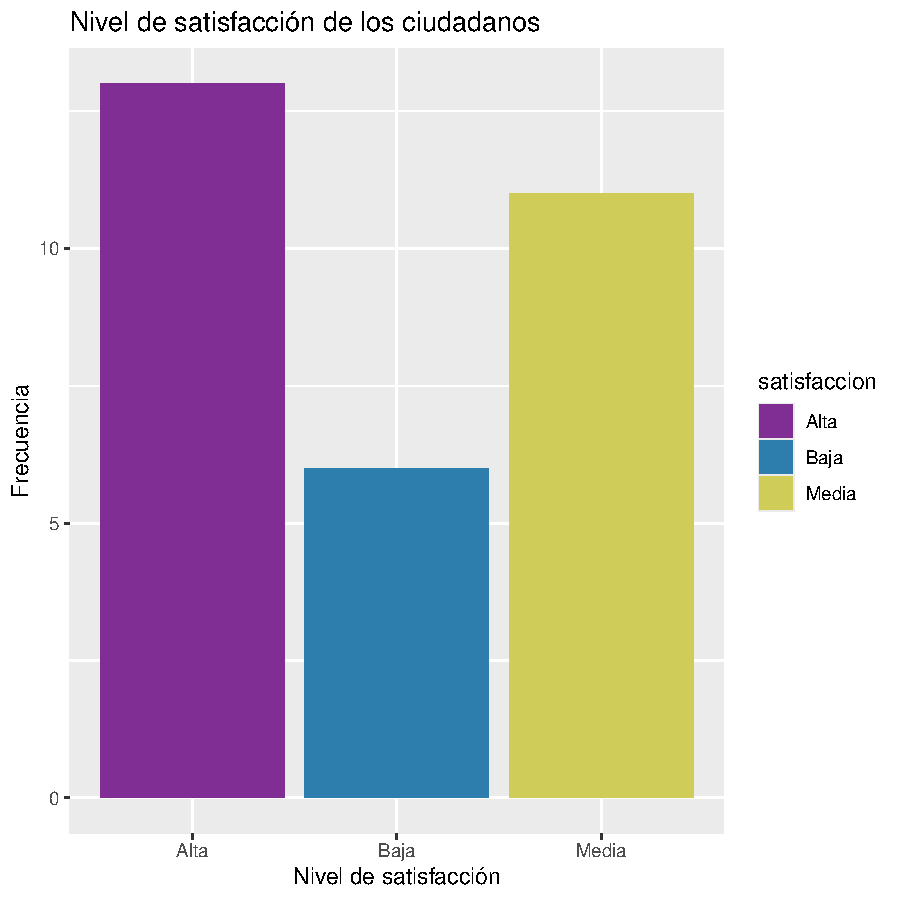
\includegraphics[width=0.7\linewidth,height=\textheight,keepaspectratio]{index_files/figure-pdf/unnamed-chunk-9-1.pdf}
\end{center}

\section{Distribución de frecuencias para datos
agrupados}\label{distribuciuxf3n-de-frecuencias-para-datos-agrupados}

Cuando una variable cuantitativa continua presenta muchos valores
diferentes, puede ser conveniente agruparlos en \textbf{intervalos de
clase}.

Por ejemplo:

\[
[20,30),\quad [30,40),\quad [40,50),\quad [50,60)
\]

Cada intervalo contiene un conjunto de valores.

\subsection{Elementos de una distribución
agrupada}\label{elementos-de-una-distribuciuxf3n-agrupada}

Para cada intervalo pueden calcularse:

\begin{itemize}
\tightlist
\item
  Límite inferior.
\item
  Límite superior.
\item
  Marca de clase.
\item
  Frecuencia absoluta.
\item
  Frecuencia acumulada.
\item
  Frecuencia relativa.
\item
  Frecuencia relativa acumulada.
\end{itemize}

La \textbf{marca de clase} se calcula mediante:

\[
x_i=\frac{L_i+U_i}{2}
\]

donde:

\begin{itemize}
\tightlist
\item
  \(L_i\) = límite inferior.
\item
  \(U_i\) = límite superior.
\end{itemize}

\section{Número de intervalos}\label{nuxfamero-de-intervalos}

Una regla frecuente para determinar aproximadamente el número de clases
es la \textbf{regla de Sturges}:

\[
k=1+3.322\log_{10}(n)
\]

donde \(n\) representa el tamaño de la muestra.

Otra expresión equivalente es:

\[
k=1+\log_2(n)
\]

Una vez determinado \(k\), puede calcularse la amplitud aproximada:

\[
A=\frac{R}{k}
\]

donde:

\[
R=X_{\max}-X_{\min}
\]

es el rango.

\section{Ejemplo con datos
cuantitativos}\label{ejemplo-con-datos-cuantitativos}

Supongamos que se dispone de los ingresos mensuales de 40 usuarios,
expresados en millones de pesos:

\begin{Shaded}
\begin{Highlighting}[]
\FunctionTok{set.seed}\NormalTok{(}\DecValTok{123}\NormalTok{)}

\NormalTok{ingresos }\OtherTok{\textless{}{-}} \FunctionTok{round}\NormalTok{(}
  \FunctionTok{runif}\NormalTok{(}\DecValTok{40}\NormalTok{, }\FloatTok{1.2}\NormalTok{, }\FloatTok{6.5}\NormalTok{),}
  \DecValTok{2}
\NormalTok{)}

\NormalTok{ingresos}
\end{Highlighting}
\end{Shaded}

\begin{verbatim}
 [1] 2.72 5.38 3.37 5.88 6.18 1.44 4.00 5.93 4.12 3.62 6.27 3.60 4.79 4.23 1.75
[16] 5.97 2.50 1.42 2.94 6.26 5.91 4.87 4.59 6.47 4.68 4.96 4.08 4.35 2.73 1.98
[31] 6.30 5.98 4.86 5.42 1.33 3.73 5.22 2.35 2.89 2.43
\end{verbatim}

Podemos construir intervalos mediante \texttt{cut()}:

\begin{Shaded}
\begin{Highlighting}[]
\NormalTok{intervalos }\OtherTok{\textless{}{-}} \FunctionTok{cut}\NormalTok{(}
\NormalTok{  ingresos,}
  \AttributeTok{breaks =} \FunctionTok{c}\NormalTok{(}\DecValTok{1}\NormalTok{, }\DecValTok{2}\NormalTok{, }\DecValTok{3}\NormalTok{, }\DecValTok{4}\NormalTok{, }\DecValTok{5}\NormalTok{, }\DecValTok{6}\NormalTok{, }\DecValTok{7}\NormalTok{),}
  \AttributeTok{right =} \ConstantTok{FALSE}
\NormalTok{)}

\FunctionTok{table}\NormalTok{(intervalos)}
\end{Highlighting}
\end{Shaded}

\begin{verbatim}
intervalos
[1,2) [2,3) [3,4) [4,5) [5,6) [6,7) 
    5     7     4    11     8     5 
\end{verbatim}

\section{Histograma}\label{histograma}

Para representar una variable cuantitativa continua:

\begin{Shaded}
\begin{Highlighting}[]
\FunctionTok{ggplot}\NormalTok{(}
  \FunctionTok{data.frame}\NormalTok{(ingresos),}
  \FunctionTok{aes}\NormalTok{(}\AttributeTok{x =}\NormalTok{ ingresos)}
\NormalTok{) }\SpecialCharTok{+}
  \FunctionTok{geom\_histogram}\NormalTok{(}
    \AttributeTok{bins =} \DecValTok{6}
\NormalTok{  ) }\SpecialCharTok{+}
  \FunctionTok{labs}\NormalTok{(}
    \AttributeTok{title =} \StringTok{"Distribución de los ingresos mensuales"}\NormalTok{,}
    \AttributeTok{x =} \StringTok{"Ingresos (millones de pesos)"}\NormalTok{,}
    \AttributeTok{y =} \StringTok{"Frecuencia"}
\NormalTok{  ) }\SpecialCharTok{+}
  \FunctionTok{theme\_minimal}\NormalTok{()}
\end{Highlighting}
\end{Shaded}

\begin{center}
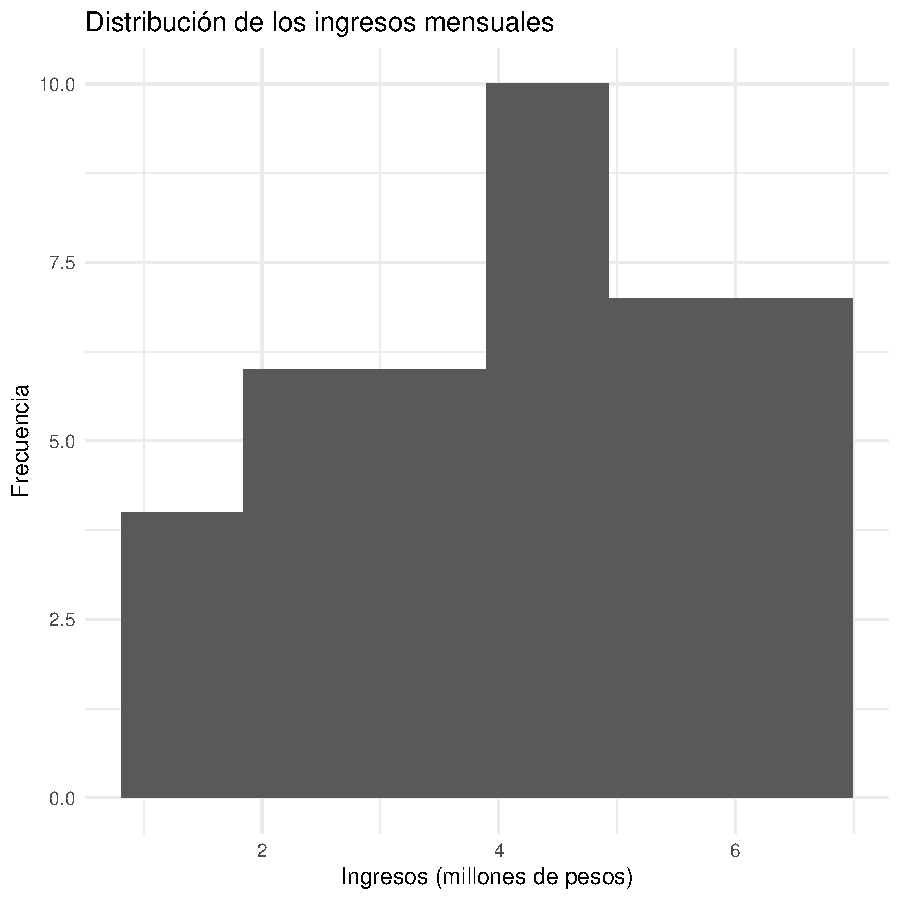
\includegraphics[width=0.7\linewidth,height=\textheight,keepaspectratio]{index_files/figure-pdf/unnamed-chunk-12-1.pdf}
\end{center}

\section{Distribución de frecuencias
bidimensional}\label{distribuciuxf3n-de-frecuencias-bidimensional}

\subsection{Concepto}\label{concepto-1}

Una \textbf{distribución de frecuencias bidimensional} estudia
simultáneamente dos variables estadísticas.

Sean:

\[
X \quad \text{y} \quad Y
\]

dos variables observadas sobre los mismos individuos.

El objetivo consiste en analizar cómo se distribuyen conjuntamente los
valores de ambas variables.

Por ejemplo:

\begin{itemize}
\tightlist
\item
  Edad y satisfacción.
\item
  Nivel educativo y satisfacción.
\item
  Estrato y acceso a un programa social.
\item
  Modalidad de atención y satisfacción.
\item
  Género y tipo de servicio utilizado.
\end{itemize}

\section{Tabla de contingencia}\label{tabla-de-contingencia}

Cuando las dos variables son cualitativas o categóricas, la distribución
bidimensional suele representarse mediante una \textbf{tabla de
contingencia}.

Supongamos que se estudian:

\begin{itemize}
\tightlist
\item
  \(X\): modalidad de atención.
\item
  \(Y\): nivel de satisfacción.
\end{itemize}

La tabla puede tener la siguiente estructura:

{\def\LTcaptype{none} % do not increment counter
\begin{longtable}[]{@{}lrrrr@{}}
\toprule\noalign{}
Modalidad & Alta & Media & Baja & Total \\
\midrule\noalign{}
\endhead
\bottomrule\noalign{}
\endlastfoot
Presencial & \(n_{11}\) & \(n_{12}\) & \(n_{13}\) & \(n_{1.}\) \\
Virtual & \(n_{21}\) & \(n_{22}\) & \(n_{23}\) & \(n_{2.}\) \\
\textbf{Total} & \(n_{.1}\) & \(n_{.2}\) & \(n_{.3}\) & \(n\) \\
\end{longtable}
}

Los valores \(n_{ij}\) representan las \textbf{frecuencias conjuntas}.

\section{Frecuencia conjunta}\label{frecuencia-conjunta}

La frecuencia conjunta \(n_{ij}\) corresponde al número de individuos
que simultáneamente presentan:

\[
X=x_i
\]

y

\[
Y=y_j
\]

Por ejemplo:

\[
n_{23}
\]

representaría el número de individuos pertenecientes a la categoría 2 de
\(X\) y a la categoría 3 de \(Y\).

\section{Frecuencias marginales}\label{frecuencias-marginales}

Las \textbf{frecuencias marginales} se obtienen sumando las frecuencias
de las filas o columnas.

\subsection{Frecuencia marginal de X}\label{frecuencia-marginal-de-x}

\[
n_{i.}=\sum_j n_{ij}
\]

\subsection{Frecuencia marginal de Y}\label{frecuencia-marginal-de-y}

\[
n_{.j}=\sum_i n_{ij}
\]

El total general es:

\[
n=\sum_i\sum_j n_{ij}
\]

\section{Frecuencias relativas
bidimensionales}\label{frecuencias-relativas-bidimensionales}

La frecuencia relativa conjunta se calcula como:

\[
h_{ij}=\frac{n_{ij}}{n}
\]

y cumple:

\[
\sum_i\sum_jh_{ij}=1
\]

En porcentaje:

\[
p_{ij}=100h_{ij}
\]

\section{Frecuencias condicionales}\label{frecuencias-condicionales}

Las frecuencias condicionales permiten analizar la distribución de una
variable \textbf{dentro de una categoría específica de la otra
variable}.

Si queremos analizar \(Y\) condicionado a \(X=x_i\):

\[
h_{j|i}=
\frac{n_{ij}}{n_{i.}}
\]

Si queremos analizar \(X\) condicionado a \(Y=y_j\):

\[
h_{i|j}=
\frac{n_{ij}}{n_{.j}}
\]

Las frecuencias condicionales son fundamentales para estudiar posibles
relaciones entre dos variables.

\section{Ejemplo de tabla bidimensional en
R}\label{ejemplo-de-tabla-bidimensional-en-r}

Consideremos una encuesta realizada a 100 ciudadanos:

\begin{Shaded}
\begin{Highlighting}[]
\NormalTok{datos }\OtherTok{\textless{}{-}} \FunctionTok{data.frame}\NormalTok{(}
  \AttributeTok{Modalidad =} \FunctionTok{c}\NormalTok{(}
    \StringTok{"Presencial"}\NormalTok{,}\StringTok{"Presencial"}\NormalTok{,}\StringTok{"Presencial"}\NormalTok{,}
    \StringTok{"Virtual"}\NormalTok{,}\StringTok{"Virtual"}\NormalTok{,}\StringTok{"Virtual"}
\NormalTok{  ),}
  \AttributeTok{Satisfaccion =} \FunctionTok{c}\NormalTok{(}
    \StringTok{"Alta"}\NormalTok{,}\StringTok{"Media"}\NormalTok{,}\StringTok{"Baja"}\NormalTok{,}
    \StringTok{"Alta"}\NormalTok{,}\StringTok{"Media"}\NormalTok{,}\StringTok{"Baja"}
\NormalTok{  ),}
  \AttributeTok{Frecuencia =} \FunctionTok{c}\NormalTok{(}
    \DecValTok{30}\NormalTok{,}\DecValTok{15}\NormalTok{,}\DecValTok{5}\NormalTok{,}
    \DecValTok{20}\NormalTok{,}\DecValTok{20}\NormalTok{,}\DecValTok{10}
\NormalTok{  )}
\NormalTok{)}

\NormalTok{datos}
\end{Highlighting}
\end{Shaded}

\begin{verbatim}
   Modalidad Satisfaccion Frecuencia
1 Presencial         Alta         30
2 Presencial        Media         15
3 Presencial         Baja          5
4    Virtual         Alta         20
5    Virtual        Media         20
6    Virtual         Baja         10
\end{verbatim}

Para obtener una tabla de contingencia:

\begin{Shaded}
\begin{Highlighting}[]
\NormalTok{tabla }\OtherTok{\textless{}{-}} \FunctionTok{xtabs}\NormalTok{(}
\NormalTok{  Frecuencia }\SpecialCharTok{\textasciitilde{}}\NormalTok{ Modalidad }\SpecialCharTok{+}\NormalTok{ Satisfaccion,}
  \AttributeTok{data =}\NormalTok{ datos}
\NormalTok{)}

\NormalTok{tabla}
\end{Highlighting}
\end{Shaded}

\begin{verbatim}
            Satisfaccion
Modalidad    Alta Baja Media
  Presencial   30    5    15
  Virtual      20   10    20
\end{verbatim}

El resultado conceptual es:

{\def\LTcaptype{none} % do not increment counter
\begin{longtable}[]{@{}lrrr@{}}
\toprule\noalign{}
Modalidad & Alta & Media & Baja \\
\midrule\noalign{}
\endhead
\bottomrule\noalign{}
\endlastfoot
Presencial & 30 & 15 & 5 \\
Virtual & 20 & 20 & 10 \\
\end{longtable}
}

\section{Totales marginales en R}\label{totales-marginales-en-r}

Podemos obtener los totales de filas y columnas mediante:

\begin{Shaded}
\begin{Highlighting}[]
\FunctionTok{addmargins}\NormalTok{(tabla)}
\end{Highlighting}
\end{Shaded}

\begin{verbatim}
            Satisfaccion
Modalidad    Alta Baja Media Sum
  Presencial   30    5    15  50
  Virtual      20   10    20  50
  Sum          50   15    35 100
\end{verbatim}

También:

\begin{Shaded}
\begin{Highlighting}[]
\FunctionTok{margin.table}\NormalTok{(tabla, }\DecValTok{1}\NormalTok{)}
\end{Highlighting}
\end{Shaded}

\begin{verbatim}
Modalidad
Presencial    Virtual 
        50         50 
\end{verbatim}

permite obtener las frecuencias marginales de las filas.

Mientras:

\begin{Shaded}
\begin{Highlighting}[]
\FunctionTok{margin.table}\NormalTok{(tabla, }\DecValTok{2}\NormalTok{)}
\end{Highlighting}
\end{Shaded}

\begin{verbatim}
Satisfaccion
 Alta  Baja Media 
   50    15    35 
\end{verbatim}

obtiene las frecuencias marginales de las columnas.

\section{Frecuencias relativas en R}\label{frecuencias-relativas-en-r}

Para obtener las frecuencias relativas conjuntas:

\begin{Shaded}
\begin{Highlighting}[]
\FunctionTok{prop.table}\NormalTok{(tabla)}
\end{Highlighting}
\end{Shaded}

\begin{verbatim}
            Satisfaccion
Modalidad    Alta Baja Media
  Presencial 0.30 0.05  0.15
  Virtual    0.20 0.10  0.20
\end{verbatim}

Para obtener porcentajes:

\begin{Shaded}
\begin{Highlighting}[]
\FunctionTok{round}\NormalTok{(}\FunctionTok{prop.table}\NormalTok{(tabla) }\SpecialCharTok{*} \DecValTok{100}\NormalTok{, }\DecValTok{2}\NormalTok{)}
\end{Highlighting}
\end{Shaded}

\begin{verbatim}
            Satisfaccion
Modalidad    Alta Baja Media
  Presencial   30    5    15
  Virtual      20   10    20
\end{verbatim}

\section{Porcentajes por fila}\label{porcentajes-por-fila}

Para estudiar la distribución de la satisfacción dentro de cada
modalidad:

\begin{Shaded}
\begin{Highlighting}[]
\FunctionTok{prop.table}\NormalTok{(tabla, }\DecValTok{1}\NormalTok{)}
\end{Highlighting}
\end{Shaded}

\begin{verbatim}
            Satisfaccion
Modalidad    Alta Baja Media
  Presencial  0.6  0.1   0.3
  Virtual     0.4  0.2   0.4
\end{verbatim}

En porcentaje:

\begin{Shaded}
\begin{Highlighting}[]
\FunctionTok{round}\NormalTok{(}\FunctionTok{prop.table}\NormalTok{(tabla, }\DecValTok{1}\NormalTok{) }\SpecialCharTok{*} \DecValTok{100}\NormalTok{, }\DecValTok{2}\NormalTok{)}
\end{Highlighting}
\end{Shaded}

\begin{verbatim}
            Satisfaccion
Modalidad    Alta Baja Media
  Presencial   60   10    30
  Virtual      40   20    40
\end{verbatim}

La opción \texttt{margin\ =\ 1} indica que los porcentajes se calculan
\textbf{por fila}.

\section{Porcentajes por columna}\label{porcentajes-por-columna}

Para estudiar la distribución de la modalidad dentro de cada nivel de
satisfacción:

\begin{Shaded}
\begin{Highlighting}[]
\FunctionTok{prop.table}\NormalTok{(tabla, }\DecValTok{2}\NormalTok{)}
\end{Highlighting}
\end{Shaded}

\begin{verbatim}
            Satisfaccion
Modalidad         Alta      Baja     Media
  Presencial 0.6000000 0.3333333 0.4285714
  Virtual    0.4000000 0.6666667 0.5714286
\end{verbatim}

En porcentaje:

\begin{Shaded}
\begin{Highlighting}[]
\FunctionTok{round}\NormalTok{(}\FunctionTok{prop.table}\NormalTok{(tabla, }\DecValTok{2}\NormalTok{) }\SpecialCharTok{*} \DecValTok{100}\NormalTok{, }\DecValTok{2}\NormalTok{)}
\end{Highlighting}
\end{Shaded}

\begin{verbatim}
            Satisfaccion
Modalidad     Alta  Baja Media
  Presencial 60.00 33.33 42.86
  Virtual    40.00 66.67 57.14
\end{verbatim}

La opción \texttt{margin\ =\ 2} indica que los porcentajes se calculan
\textbf{por columna}.

\section{Interpretación de una tabla
bidimensional}\label{interpretaciuxf3n-de-una-tabla-bidimensional}

Supongamos que para los usuarios de modalidad presencial se obtiene:

{\def\LTcaptype{none} % do not increment counter
\begin{longtable}[]{@{}lrrr@{}}
\toprule\noalign{}
Modalidad & Alta & Media & Baja \\
\midrule\noalign{}
\endhead
\bottomrule\noalign{}
\endlastfoot
Presencial & 30 & 15 & 5 \\
\end{longtable}
}

El total de usuarios presenciales es:

\[
30+15+5=50
\]

Por tanto, la proporción de usuarios presenciales con satisfacción alta
es:

\[
\frac{30}{50}=0.60
\]

o:

\[
60\%
\]

Una interpretación estadística sería:

\begin{quote}
El 60 \% de los usuarios atendidos mediante la modalidad presencial
presenta un nivel de satisfacción alto.
\end{quote}

Es importante distinguir este resultado de un porcentaje calculado sobre
el total general de la muestra.

\section{Visualización de una distribución
bidimensional}\label{visualizaciuxf3n-de-una-distribuciuxf3n-bidimensional}

Una tabla de contingencia puede representarse mediante un gráfico de
barras.

\begin{Shaded}
\begin{Highlighting}[]
\FunctionTok{library}\NormalTok{(ggplot2)}

\NormalTok{datos\_grafico }\OtherTok{\textless{}{-}} \FunctionTok{data.frame}\NormalTok{(}
  \AttributeTok{Modalidad =} \FunctionTok{rep}\NormalTok{(}
    \FunctionTok{c}\NormalTok{(}\StringTok{"Presencial"}\NormalTok{, }\StringTok{"Virtual"}\NormalTok{),}
    \AttributeTok{each =} \DecValTok{3}
\NormalTok{  ),}
  \AttributeTok{Satisfaccion =} \FunctionTok{rep}\NormalTok{(}
    \FunctionTok{c}\NormalTok{(}\StringTok{"Alta"}\NormalTok{, }\StringTok{"Media"}\NormalTok{, }\StringTok{"Baja"}\NormalTok{),}
    \DecValTok{2}
\NormalTok{  ),}
  \AttributeTok{Frecuencia =} \FunctionTok{c}\NormalTok{(}
    \DecValTok{30}\NormalTok{,}\DecValTok{15}\NormalTok{,}\DecValTok{5}\NormalTok{,}
    \DecValTok{20}\NormalTok{,}\DecValTok{20}\NormalTok{,}\DecValTok{10}
\NormalTok{  )}
\NormalTok{)}

\FunctionTok{ggplot}\NormalTok{(}
\NormalTok{  datos\_grafico,}
  \FunctionTok{aes}\NormalTok{(}
    \AttributeTok{x =}\NormalTok{ Modalidad,}
    \AttributeTok{y =}\NormalTok{ Frecuencia,}
    \AttributeTok{fill =}\NormalTok{ Satisfaccion}
\NormalTok{  )}
\NormalTok{) }\SpecialCharTok{+}
  \FunctionTok{geom\_col}\NormalTok{(}
    \AttributeTok{position =} \StringTok{"dodge"}
\NormalTok{  ) }\SpecialCharTok{+}
  \FunctionTok{labs}\NormalTok{(}
    \AttributeTok{title =} \StringTok{"Satisfacción según modalidad de atención"}\NormalTok{,}
    \AttributeTok{x =} \StringTok{"Modalidad"}\NormalTok{,}
    \AttributeTok{y =} \StringTok{"Frecuencia"}
\NormalTok{  ) }\SpecialCharTok{+}
  \FunctionTok{theme\_minimal}\NormalTok{()}
\end{Highlighting}
\end{Shaded}

\begin{center}
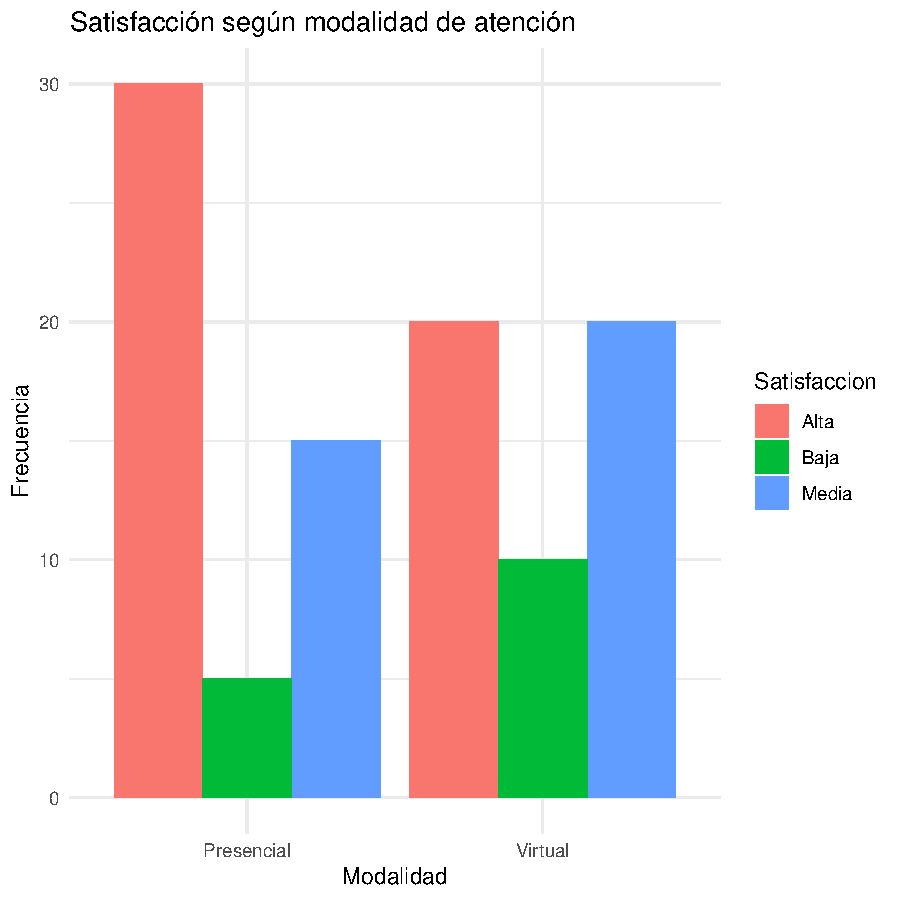
\includegraphics[width=0.7\linewidth,height=\textheight,keepaspectratio]{index_files/figure-pdf/unnamed-chunk-24-1.pdf}
\end{center}

\section{Gráfico de barras
apiladas}\label{gruxe1fico-de-barras-apiladas}

También puede utilizarse:

\begin{Shaded}
\begin{Highlighting}[]
\FunctionTok{ggplot}\NormalTok{(}
\NormalTok{  datos\_grafico,}
  \FunctionTok{aes}\NormalTok{(}
    \AttributeTok{x =}\NormalTok{ Modalidad,}
    \AttributeTok{y =}\NormalTok{ Frecuencia,}
    \AttributeTok{fill =}\NormalTok{ Satisfaccion}
\NormalTok{  )}
\NormalTok{) }\SpecialCharTok{+}
  \FunctionTok{geom\_col}\NormalTok{() }\SpecialCharTok{+}
  \FunctionTok{labs}\NormalTok{(}
    \AttributeTok{title =} \StringTok{"Distribución de la satisfacción según modalidad"}\NormalTok{,}
    \AttributeTok{x =} \StringTok{"Modalidad"}\NormalTok{,}
    \AttributeTok{y =} \StringTok{"Frecuencia"}
\NormalTok{  ) }\SpecialCharTok{+}
  \FunctionTok{theme\_minimal}\NormalTok{()}
\end{Highlighting}
\end{Shaded}

\begin{center}
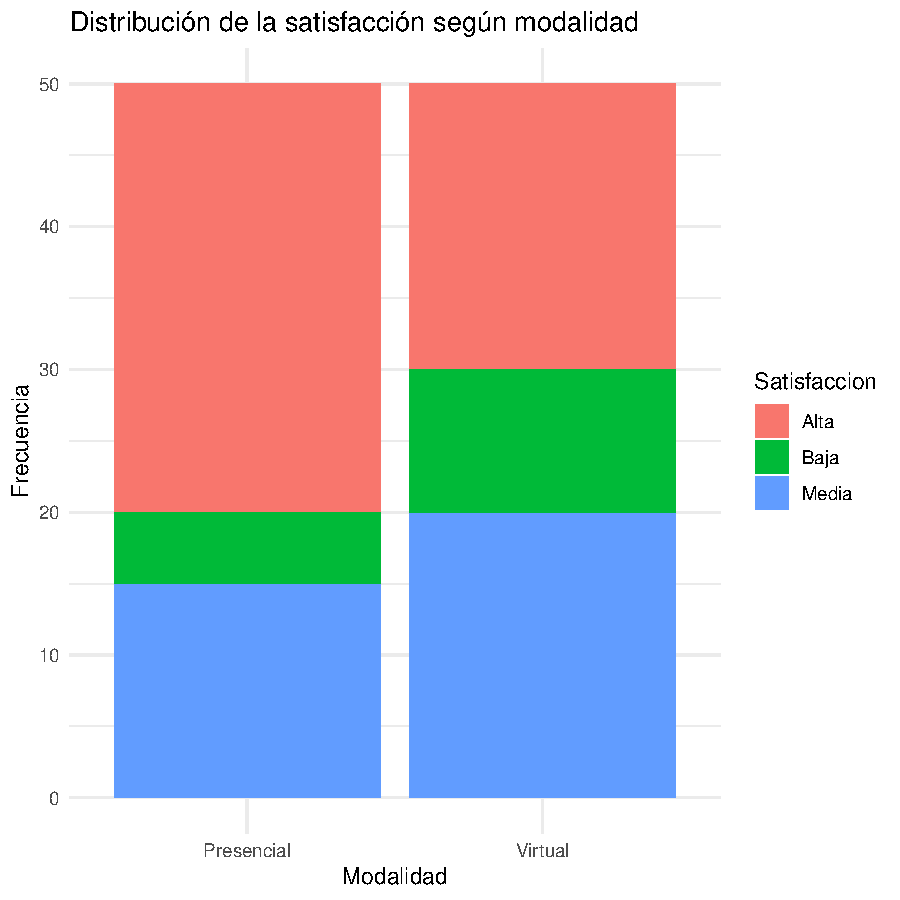
\includegraphics[width=0.7\linewidth,height=\textheight,keepaspectratio]{index_files/figure-pdf/unnamed-chunk-25-1.pdf}
\end{center}

\section{Barras proporcionales}\label{barras-proporcionales}

Para comparar estructuras porcentuales entre grupos:

\begin{Shaded}
\begin{Highlighting}[]
\FunctionTok{ggplot}\NormalTok{(}
\NormalTok{  datos\_grafico,}
  \FunctionTok{aes}\NormalTok{(}
    \AttributeTok{x =}\NormalTok{ Modalidad,}
    \AttributeTok{y =}\NormalTok{ Frecuencia,}
    \AttributeTok{fill =}\NormalTok{ Satisfaccion}
\NormalTok{  )}
\NormalTok{) }\SpecialCharTok{+}
  \FunctionTok{geom\_col}\NormalTok{(}
    \AttributeTok{position =} \StringTok{"fill"}
\NormalTok{  ) }\SpecialCharTok{+}
  \FunctionTok{scale\_y\_continuous}\NormalTok{(}
    \AttributeTok{labels =}\NormalTok{ scales}\SpecialCharTok{::}\NormalTok{percent}
\NormalTok{  ) }\SpecialCharTok{+}
  \FunctionTok{labs}\NormalTok{(}
    \AttributeTok{title =} \StringTok{"Distribución porcentual de la satisfacción"}\NormalTok{,}
    \AttributeTok{x =} \StringTok{"Modalidad"}\NormalTok{,}
    \AttributeTok{y =} \StringTok{"Porcentaje"}
\NormalTok{  ) }\SpecialCharTok{+}
  \FunctionTok{theme\_minimal}\NormalTok{()}
\end{Highlighting}
\end{Shaded}

\begin{center}
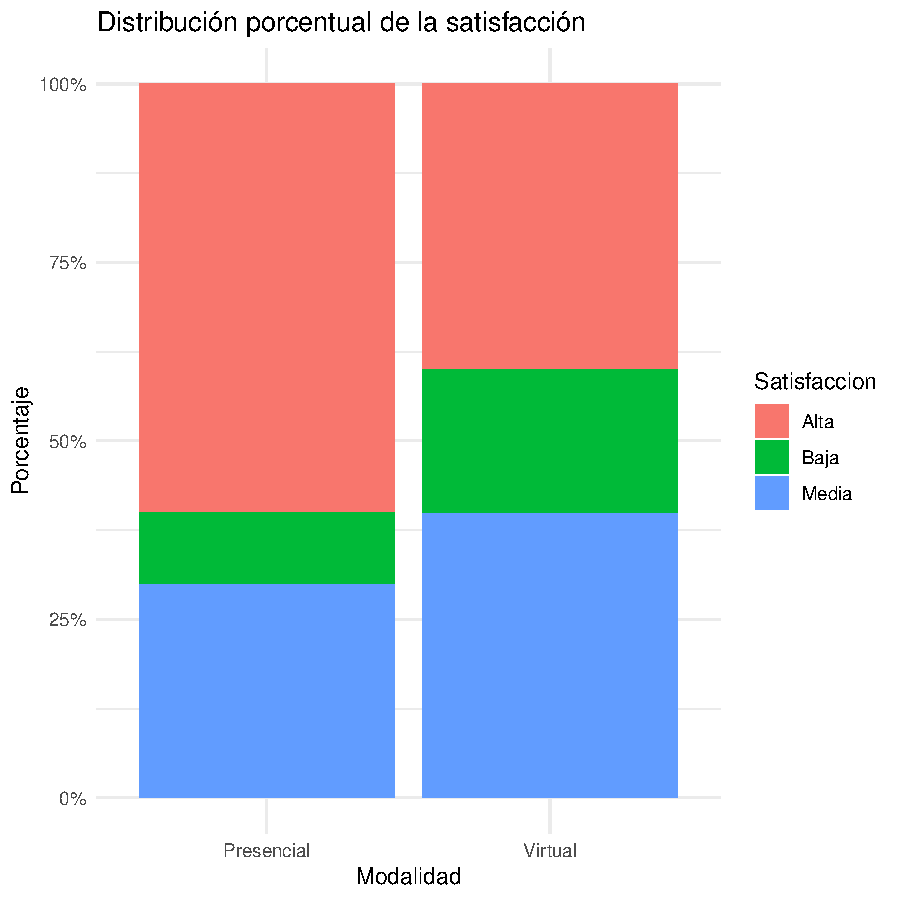
\includegraphics[width=0.7\linewidth,height=\textheight,keepaspectratio]{index_files/figure-pdf/unnamed-chunk-26-1.pdf}
\end{center}

Este gráfico resulta especialmente útil cuando los tamaños de los grupos
son diferentes.

\section{Distribución bidimensional y
asociación}\label{distribuciuxf3n-bidimensional-y-asociaciuxf3n}

Una de las principales aplicaciones de las tablas bidimensionales
consiste en estudiar si existe una posible \textbf{relación o asociación
entre dos variables}.

Por ejemplo:

\[
\text{Modalidad de atención}
\quad\longleftrightarrow\quad
\text{Satisfacción}
\]

Si las distribuciones condicionales son muy diferentes entre las
modalidades, puede existir evidencia descriptiva de asociación.

Sin embargo, una diferencia descriptiva no significa necesariamente que
exista una asociación estadísticamente significativa.

Para evaluar formalmente la asociación entre dos variables categóricas
puede utilizarse, entre otras herramientas, la \textbf{prueba
chi-cuadrado de independencia}.

\section{Prueba chi-cuadrado en R}\label{prueba-chi-cuadrado-en-r}

A partir de una tabla de contingencia:

\begin{Shaded}
\begin{Highlighting}[]
\FunctionTok{chisq.test}\NormalTok{(tabla)}
\end{Highlighting}
\end{Shaded}

\begin{verbatim}

    Pearson's Chi-squared test

data:  tabla
X-squared = 4.381, df = 2, p-value = 0.1119
\end{verbatim}

La hipótesis nula es:

\[
H_0:
\text{Las variables son independientes}
\]

Mientras que la hipótesis alternativa es:

\[
H_1:
\text{Las variables no son independientes}
\]

La decisión estadística se basa generalmente en el valor-p.

Si:

\[
p<\alpha
\]

se rechaza \(H_0\).

Si:

\[
p\geq\alpha
\]

no se rechaza \(H_0\).

Es habitual utilizar:

\[
\alpha=0.05
\]

\section{Diferencia entre distribución unidimensional y
bidimensional}\label{diferencia-entre-distribuciuxf3n-unidimensional-y-bidimensional}

{\def\LTcaptype{none} % do not increment counter
\begin{longtable}[]{@{}
  >{\raggedright\arraybackslash}p{(\linewidth - 4\tabcolsep) * \real{0.2817}}
  >{\raggedright\arraybackslash}p{(\linewidth - 4\tabcolsep) * \real{0.2817}}
  >{\raggedright\arraybackslash}p{(\linewidth - 4\tabcolsep) * \real{0.4366}}@{}}
\toprule\noalign{}
\begin{minipage}[b]{\linewidth}\raggedright
Característica
\end{minipage} & \begin{minipage}[b]{\linewidth}\raggedright
Unidimensional
\end{minipage} & \begin{minipage}[b]{\linewidth}\raggedright
Bidimensional
\end{minipage} \\
\midrule\noalign{}
\endhead
\bottomrule\noalign{}
\endlastfoot
Número de variables & 1 & 2 \\
Objetivo & Describir una variable & Analizar dos variables
conjuntamente \\
Tabla principal & Tabla de frecuencias & Tabla de contingencia \\
Frecuencia & \(f_i\) & \(n_{ij}\) \\
Frecuencia marginal & No aplica & Sí \\
Frecuencia conjunta & No aplica & Sí \\
Frecuencia condicional & No aplica & Sí \\
Asociación & No & Sí \\
Chi-cuadrado & No necesariamente & Sí, para variables categóricas \\
\end{longtable}
}

\section{Funciones fundamentales de
R}\label{funciones-fundamentales-de-r}

Las siguientes funciones son especialmente útiles para trabajar con
distribuciones de frecuencias:

{\def\LTcaptype{none} % do not increment counter
\begin{longtable}[]{@{}ll@{}}
\toprule\noalign{}
Función & Utilidad \\
\midrule\noalign{}
\endhead
\bottomrule\noalign{}
\endlastfoot
\texttt{table()} & Frecuencias absolutas \\
\texttt{prop.table()} & Frecuencias relativas \\
\texttt{cumsum()} & Frecuencias acumuladas \\
\texttt{xtabs()} & Tablas de contingencia \\
\texttt{addmargins()} & Totales marginales \\
\texttt{margin.table()} & Frecuencias marginales \\
\texttt{cut()} & Agrupar variables cuantitativas \\
\texttt{ggplot()} & Visualización \\
\texttt{geom\_bar()} & Gráfico de barras \\
\texttt{geom\_col()} & Barras con frecuencias existentes \\
\texttt{geom\_histogram()} & Histograma \\
\texttt{chisq.test()} & Prueba chi-cuadrado \\
\end{longtable}
}

\section{Función general para construir una tabla de
frecuencias}\label{funciuxf3n-general-para-construir-una-tabla-de-frecuencias}

En R podemos crear una función reutilizable:

\begin{Shaded}
\begin{Highlighting}[]
\NormalTok{tabla\_frecuencias }\OtherTok{\textless{}{-}} \ControlFlowTok{function}\NormalTok{(x) \{}
  
\NormalTok{  fi }\OtherTok{\textless{}{-}} \FunctionTok{table}\NormalTok{(x)}
  
\NormalTok{  tabla }\OtherTok{\textless{}{-}} \FunctionTok{data.frame}\NormalTok{(}
    \AttributeTok{Valor =} \FunctionTok{names}\NormalTok{(fi),}
    \AttributeTok{fi =} \FunctionTok{as.vector}\NormalTok{(fi)}
\NormalTok{  )}
  
\NormalTok{  tabla}\SpecialCharTok{$}\NormalTok{Fi }\OtherTok{\textless{}{-}} \FunctionTok{cumsum}\NormalTok{(tabla}\SpecialCharTok{$}\NormalTok{fi)}
  
\NormalTok{  tabla}\SpecialCharTok{$}\NormalTok{hi }\OtherTok{\textless{}{-}}\NormalTok{ tabla}\SpecialCharTok{$}\NormalTok{fi }\SpecialCharTok{/} \FunctionTok{sum}\NormalTok{(tabla}\SpecialCharTok{$}\NormalTok{fi)}
  
\NormalTok{  tabla}\SpecialCharTok{$}\NormalTok{Hi }\OtherTok{\textless{}{-}} \FunctionTok{cumsum}\NormalTok{(tabla}\SpecialCharTok{$}\NormalTok{hi)}
  
\NormalTok{  tabla}\SpecialCharTok{$}\NormalTok{Porcentaje }\OtherTok{\textless{}{-}}\NormalTok{ tabla}\SpecialCharTok{$}\NormalTok{hi }\SpecialCharTok{*} \DecValTok{100}
  
\NormalTok{  tabla}
\NormalTok{\}}
\end{Highlighting}
\end{Shaded}

Aplicación:

\begin{Shaded}
\begin{Highlighting}[]
\FunctionTok{tabla\_frecuencias}\NormalTok{(satisfaccion)}
\end{Highlighting}
\end{Shaded}

\begin{verbatim}
  Valor fi Fi        hi        Hi Porcentaje
1  Alta 13 13 0.4333333 0.4333333   43.33333
2  Baja  6 19 0.2000000 0.6333333   20.00000
3 Media 11 30 0.3666667 1.0000000   36.66667
\end{verbatim}

\section{Recomendaciones para el análisis
estadístico}\label{recomendaciones-para-el-anuxe1lisis-estaduxedstico}

Al construir e interpretar una distribución de frecuencias es
importante:

\begin{enumerate}
\def\labelenumi{\arabic{enumi}.}
\tightlist
\item
  Identificar correctamente el tipo de variable.
\item
  Diferenciar variables cualitativas y cuantitativas.
\item
  Utilizar frecuencias absolutas cuando interesa conocer cantidades.
\item
  Utilizar frecuencias relativas o porcentajes cuando se desean comparar
  grupos.
\item
  Emplear frecuencias acumuladas cuando la variable posee un orden
  natural.
\item
  Para datos continuos con muchos valores, considerar agrupación en
  intervalos.
\item
  En tablas bidimensionales, especificar claramente si los porcentajes
  se calculan por filas, columnas o sobre el total.
\item
  Complementar las tablas con representaciones gráficas apropiadas.
\item
  No confundir asociación descriptiva con causalidad.
\item
  Cuando sea pertinente, complementar el análisis descriptivo con
  pruebas estadísticas.
\end{enumerate}

\section{Ejemplo aplicado a la Administración
Pública}\label{ejemplo-aplicado-a-la-administraciuxf3n-puxfablica}

Supongamos que una entidad territorial realiza una encuesta a ciudadanos
para estudiar la satisfacción con un servicio público.

Se registran las variables:

\begin{itemize}
\tightlist
\item
  \texttt{Edad}
\item
  \texttt{Modalidad}
\item
  \texttt{Satisfaccion}
\item
  \texttt{Estrato}
\item
  \texttt{Numero\_tramites}
\end{itemize}

Una distribución unidimensional puede responder:

\begin{quote}
¿Cuál es el nivel de satisfacción predominante entre los ciudadanos?
\end{quote}

Mientras que una distribución bidimensional puede responder:

\begin{quote}
¿Cómo se distribuye el nivel de satisfacción según la modalidad de
atención?
\end{quote}

La primera pregunta utiliza una \textbf{distribución de frecuencias
unidimensional}.

La segunda utiliza una \textbf{distribución de frecuencias
bidimensional}.

\section{Flujo de trabajo recomendado en
RStudio}\label{flujo-de-trabajo-recomendado-en-rstudio}

Un análisis profesional puede seguir la siguiente secuencia:

\begin{Shaded}
\begin{Highlighting}[]
\NormalTok{Importación de datos}
\NormalTok{        ↓}
\NormalTok{Exploración de variables}
\NormalTok{        ↓}
\NormalTok{Identificación del tipo de variable}
\NormalTok{        ↓}
\NormalTok{Distribución unidimensional}
\NormalTok{        ↓}
\NormalTok{Frecuencias absolutas y relativas}
\NormalTok{        ↓}
\NormalTok{Representación gráfica}
\NormalTok{        ↓}
\NormalTok{Distribución bidimensional}
\NormalTok{        ↓}
\NormalTok{Frecuencias conjuntas y marginales}
\NormalTok{        ↓}
\NormalTok{Porcentajes condicionales}
\NormalTok{        ↓}
\NormalTok{Representación gráfica}
\NormalTok{        ↓}
\NormalTok{Análisis de asociación}
\NormalTok{        ↓}
\NormalTok{Interpretación estadística}
\end{Highlighting}
\end{Shaded}

\section{Conclusiones}\label{conclusiones}

Las \textbf{distribuciones de frecuencias unidimensionales} permiten
organizar y resumir la información correspondiente a una sola variable
mediante frecuencias absolutas, acumuladas, relativas y porcentuales.

Las \textbf{distribuciones de frecuencias bidimensionales} permiten
analizar conjuntamente dos variables y constituyen una herramienta
fundamental para estudiar patrones de asociación mediante frecuencias
conjuntas, marginales y condicionales.

En \textbf{R/RStudio}, funciones como \texttt{table()},
\texttt{prop.table()}, \texttt{cumsum()}, \texttt{xtabs()} y
\texttt{ggplot2} permiten automatizar gran parte del proceso de
construcción, análisis y visualización de las distribuciones de
frecuencias.

El análisis estadístico debe ir más allá de la construcción mecánica de
tablas: es fundamental interpretar los resultados dentro del contexto de
investigación y seleccionar correctamente los porcentajes, gráficos y
procedimientos estadísticos de acuerdo con el tipo de variables
estudiadas.

\section{Resumen de fórmulas}\label{resumen-de-fuxf3rmulas}

\subsection{Frecuencia absoluta}\label{frecuencia-absoluta-1}

\[
f_i
\]

\subsection{Frecuencia absoluta
acumulada}\label{frecuencia-absoluta-acumulada-1}

\[
F_i=\sum_{j=1}^{i}f_j
\]

\subsection{Frecuencia relativa}\label{frecuencia-relativa-1}

\[
h_i=\frac{f_i}{n}
\]

\subsection{Frecuencia relativa
acumulada}\label{frecuencia-relativa-acumulada-1}

\[
H_i=\sum_{j=1}^{i}h_j
\]

\subsection{Porcentaje}\label{porcentaje}

\[
p_i=100h_i
\]

\subsection{Frecuencia conjunta}\label{frecuencia-conjunta-1}

\[
n_{ij}
\]

\subsection{Frecuencia marginal de X}\label{frecuencia-marginal-de-x-1}

\[
n_{i.}=\sum_jn_{ij}
\]

\subsection{Frecuencia marginal de Y}\label{frecuencia-marginal-de-y-1}

\[
n_{.j}=\sum_in_{ij}
\]

\subsection{Frecuencia relativa
conjunta}\label{frecuencia-relativa-conjunta}

\[
h_{ij}=\frac{n_{ij}}{n}
\]

\subsection{Frecuencia condicional}\label{frecuencia-condicional}

\[
h_{j|i}=\frac{n_{ij}}{n_{i.}}
\]

\subsection{Regla de Sturges}\label{regla-de-sturges}

\[
k=1+3.322\log_{10}(n)
\]

\subsection{Amplitud}\label{amplitud}

\[
A=\frac{R}{k}
\]

\subsection{Rango}\label{rango}

\[
R=X_{\max}-X_{\min}
\]

\subsection{Marca de clase}\label{marca-de-clase}

\[
x_i=\frac{L_i+U_i}{2}
\]




\end{document}
